\documentclass[a4paper]{book}
\usepackage{a4wide}
\usepackage{makeidx}
\usepackage{fancyhdr}
\usepackage{graphicx}
\usepackage{multicol}
\usepackage{float}
\usepackage{textcomp}
\usepackage{alltt}
\usepackage{times}
\usepackage{ifpdf}
\ifpdf
\usepackage[pdftex,
            pagebackref=true,
            colorlinks=true,
            linkcolor=blue,
            unicode
           ]{hyperref}
\else
\usepackage[ps2pdf,
            pagebackref=true,
            colorlinks=true,
            linkcolor=blue,
            unicode
           ]{hyperref}
\usepackage{pspicture}
\fi
\usepackage[utf8]{inputenc}
\usepackage{doxygen}
\makeindex
\setcounter{tocdepth}{3}
\renewcommand{\footrulewidth}{0.4pt}
\begin{document}
\begin{titlepage}
\vspace*{7cm}
\begin{center}
{\Large Domogik }\\
\vspace*{1cm}
{\large Generated by Doxygen 1.5.6}\\
\vspace*{0.5cm}
{\small Thu Feb 5 11:25:04 2009}\\
\end{center}
\end{titlepage}
\clearemptydoublepage
\pagenumbering{roman}
\tableofcontents
\clearemptydoublepage
\pagenumbering{arabic}
\chapter{Directory Hierarchy}
\section{Directories}
This directory hierarchy is sorted roughly, but not completely, alphabetically:\begin{CompactList}
\item \contentsline{section}{common}{\pageref{dir_55355cdeea956e0ff37897760d49a8b7}}{}
\item \contentsline{section}{config}{\pageref{dir_cee9c79587f570ceb8ce290779602f9e}}{}
\item \contentsline{section}{control}{\pageref{dir_ab51fe5183395bffca5b27dcaf8dba7d}}{}
\item \contentsline{section}{xpl}{\pageref{dir_bcacd883f70269073ed4fd6ad0018512}}{}
\end{CompactList}

\chapter{Class Index}
\section{Class Hierarchy}
This inheritance list is sorted roughly, but not completely, alphabetically:\begin{CompactList}
\item \contentsline{section}{domogik::xpl::trigger::Condition}{\pageref{classdomogik_1_1xpl_1_1trigger_1_1Condition}}{}
\begin{CompactList}
\item \contentsline{section}{domogik::xpl::trigger::AND}{\pageref{classdomogik_1_1xpl_1_1trigger_1_1AND}}{}
\item \contentsline{section}{domogik::xpl::trigger::NOT}{\pageref{classdomogik_1_1xpl_1_1trigger_1_1NOT}}{}
\item \contentsline{section}{domogik::xpl::trigger::OR}{\pageref{classdomogik_1_1xpl_1_1trigger_1_1OR}}{}
\item \contentsline{section}{domogik::xpl::trigger::stateCond}{\pageref{classdomogik_1_1xpl_1_1trigger_1_1stateCond}}{}
\item \contentsline{section}{domogik::xpl::trigger::timeCond}{\pageref{classdomogik_1_1xpl_1_1trigger_1_1timeCond}}{}
\end{CompactList}
\item \contentsline{section}{generate\_\-config::ConfigManager}{\pageref{classgenerate__config_1_1ConfigManager}}{}
\item \contentsline{section}{domogik::control::models::DeviceCategory}{\pageref{classdomogik_1_1control_1_1models_1_1DeviceCategory}}{}
\item \contentsline{section}{domogik::doxypy::FSM}{\pageref{classdomogik_1_1doxypy_1_1FSM}}{}
\item \contentsline{section}{generate\_\-config::genericPluginConfig}{\pageref{classgenerate__config_1_1genericPluginConfig}}{}
\begin{CompactList}
\item \contentsline{section}{generate\_\-config::datetimeConfig}{\pageref{classgenerate__config_1_1datetimeConfig}}{}
\item \contentsline{section}{generate\_\-config::generalConfig}{\pageref{classgenerate__config_1_1generalConfig}}{}
\item \contentsline{section}{generate\_\-config::senderConfig}{\pageref{classgenerate__config_1_1senderConfig}}{}
\item \contentsline{section}{generate\_\-config::triggerConfig}{\pageref{classgenerate__config_1_1triggerConfig}}{}
\item \contentsline{section}{generate\_\-config::x10Config}{\pageref{classgenerate__config_1_1x10Config}}{}
\end{CompactList}
\item \contentsline{section}{domogik::xpl::xPLAPI::Listener}{\pageref{classdomogik_1_1xpl_1_1xPLAPI_1_1Listener}}{}
\item \contentsline{section}{domogik::xpl::trigger::ListenerBuilder}{\pageref{classdomogik_1_1xpl_1_1trigger_1_1ListenerBuilder}}{}
\item \contentsline{section}{domogik::common::configloader::Loader}{\pageref{classdomogik_1_1common_1_1configloader_1_1Loader}}{}
\item \contentsline{section}{domogik::common::logger::Logger}{\pageref{classdomogik_1_1common_1_1logger_1_1Logger}}{}
\item \contentsline{section}{domogik::xpl::xPLAPI::Manager}{\pageref{classdomogik_1_1xpl_1_1xPLAPI_1_1Manager}}{}
\item \contentsline{section}{domogik::xpl::xPLAPI::Message}{\pageref{classdomogik_1_1xpl_1_1xPLAPI_1_1Message}}{}
\item \contentsline{section}{domogik::xpl::onewire::OneWire}{\pageref{classdomogik_1_1xpl_1_1onewire_1_1OneWire}}{}
\item \contentsline{section}{domogik::xpl::onewire::OneWireException}{\pageref{classdomogik_1_1xpl_1_1onewire_1_1OneWireException}}{}
\item \contentsline{section}{domogik::control::SampleDataHelper::SampleDataHelper}{\pageref{classdomogik_1_1control_1_1SampleDataHelper_1_1SampleDataHelper}}{}
\item \contentsline{section}{domogik::xpl::x10API::X10API}{\pageref{classdomogik_1_1xpl_1_1x10API_1_1X10API}}{}
\item \contentsline{section}{domogik::xpl::x10API::X10Exception}{\pageref{classdomogik_1_1xpl_1_1x10API_1_1X10Exception}}{}
\item \contentsline{section}{domogik::xpl::datetime::xPLDateTime}{\pageref{classdomogik_1_1xpl_1_1datetime_1_1xPLDateTime}}{}
\item \contentsline{section}{domogik::xpl::xPLAPI::XPLException}{\pageref{classdomogik_1_1xpl_1_1xPLAPI_1_1XPLException}}{}
\item \contentsline{section}{domogik::control::XPLHelper::XPLHelper}{\pageref{classdomogik_1_1control_1_1XPLHelper_1_1XPLHelper}}{}
\item \contentsline{section}{domogik::xpl::xPLAPI::xPLTimer}{\pageref{classdomogik_1_1xpl_1_1xPLAPI_1_1xPLTimer}}{}
\end{CompactList}

\chapter{Class Index}
\section{Class List}
Here are the classes, structs, unions and interfaces with brief descriptions:\begin{CompactList}
\item\contentsline{section}{\hyperlink{classtrigger_1_1AND}{trigger::AND} (Implementation for the \hyperlink{classtrigger_1_1AND}{AND} operator )}{\pageref{classtrigger_1_1AND}}{}
\item\contentsline{section}{\hyperlink{classtrigger_1_1Condition}{trigger::Condition} (Parent class for each condition A condition can be a node : it store 1 or 2 other conditions, or a final node : it just implements some eval of the condition )}{\pageref{classtrigger_1_1Condition}}{}
\item\contentsline{section}{\hyperlink{classgenerate__config_1_1ConfigManager}{generate\_\-config::ConfigManager} (General config manager which can ask user about config settings, check results and write config file )}{\pageref{classgenerate__config_1_1ConfigManager}}{}
\item\contentsline{section}{\hyperlink{classgenerate__config_1_1datetimeConfig}{generate\_\-config::datetimeConfig} (Ask the user for specific config for the xPL datetime module )}{\pageref{classgenerate__config_1_1datetimeConfig}}{}
\item\contentsline{section}{\hyperlink{classdomogik_1_1doxypy_1_1FSM}{domogik::doxypy::FSM} (Implements a finite state machine )}{\pageref{classdomogik_1_1doxypy_1_1FSM}}{}
\item\contentsline{section}{\hyperlink{classgenerate__config_1_1generalConfig}{generate\_\-config::generalConfig} (Ask the user for general configuration and write results )}{\pageref{classgenerate__config_1_1generalConfig}}{}
\item\contentsline{section}{\hyperlink{classgenerate__config_1_1genericPluginConfig}{generate\_\-config::genericPluginConfig} (Generic list for plugins )}{\pageref{classgenerate__config_1_1genericPluginConfig}}{}
\item\contentsline{section}{\hyperlink{classxPLAPI_1_1Listener}{xPLAPI::Listener} (\hyperlink{classxPLAPI_1_1Listener}{Listener} are objects which are able to check if a message match some filter and to call a function if they do )}{\pageref{classxPLAPI_1_1Listener}}{}
\item\contentsline{section}{\hyperlink{classtrigger_1_1ListenerBuilder}{trigger::ListenerBuilder} (Class to parse an expression and create appropriated listener )}{\pageref{classtrigger_1_1ListenerBuilder}}{}
\item\contentsline{section}{\hyperlink{classconfigloader_1_1Loader}{configloader::Loader} (Parse Domogik config files )}{\pageref{classconfigloader_1_1Loader}}{}
\item\contentsline{section}{\hyperlink{classxPLAPI_1_1Manager}{xPLAPI::Manager} (\hyperlink{classxPLAPI_1_1Manager}{Manager} is the main component of the system You can run many managers on different port Each manager will send an heartbeat message on broadcast on port 3865 to announce itself to the xPL Hub )}{\pageref{classxPLAPI_1_1Manager}}{}
\item\contentsline{section}{\hyperlink{classxPLAPI_1_1Message}{xPLAPI::Message} (\hyperlink{classxPLAPI_1_1Message}{Message} is the object for all data received form the network )}{\pageref{classxPLAPI_1_1Message}}{}
\item\contentsline{section}{\hyperlink{classtrigger_1_1NOT}{trigger::NOT} (Implementation for the \hyperlink{classtrigger_1_1NOT}{NOT} operator )}{\pageref{classtrigger_1_1NOT}}{}
\item\contentsline{section}{\hyperlink{classonewire_1_1OneWire}{onewire::OneWire} (Manage \hyperlink{classonewire_1_1OneWire}{OneWire} )}{\pageref{classonewire_1_1OneWire}}{}
\item\contentsline{section}{\hyperlink{classonewire_1_1OneWireException}{onewire::OneWireException} (\hyperlink{classonewire_1_1OneWire}{OneWire} exception )}{\pageref{classonewire_1_1OneWireException}}{}
\item\contentsline{section}{\hyperlink{classtrigger_1_1OR}{trigger::OR} (Implementation for the \hyperlink{classtrigger_1_1OR}{OR} operator )}{\pageref{classtrigger_1_1OR}}{}
\item\contentsline{section}{\hyperlink{classdomogik_1_1control_1_1SampleDataHelper_1_1SampleDataHelper}{domogik::control::SampleDataHelper::SampleDataHelper} (Class to load / clear sample data )}{\pageref{classdomogik_1_1control_1_1SampleDataHelper_1_1SampleDataHelper}}{}
\item\contentsline{section}{\hyperlink{classgenerate__config_1_1senderConfig}{generate\_\-config::senderConfig} (Ask the user for specific config for the xPL sender )}{\pageref{classgenerate__config_1_1senderConfig}}{}
\item\contentsline{section}{\hyperlink{classtrigger_1_1stateCond}{trigger::stateCond} (Implementation of the state condition This allows user to describe a condition on any item of the system )}{\pageref{classtrigger_1_1stateCond}}{}
\item\contentsline{section}{\hyperlink{classtrigger_1_1timeCond}{trigger::timeCond} (Implementation of the time condition This allows user to describe time periods like cron )}{\pageref{classtrigger_1_1timeCond}}{}
\item\contentsline{section}{\hyperlink{classgenerate__config_1_1triggerConfig}{generate\_\-config::triggerConfig} (Ask the user for specific config for the xPL sender )}{\pageref{classgenerate__config_1_1triggerConfig}}{}
\item\contentsline{section}{\hyperlink{classx10API_1_1X10API}{x10API::X10API} (This class define some facilities to use X10 )}{\pageref{classx10API_1_1X10API}}{}
\item\contentsline{section}{\hyperlink{classgenerate__config_1_1x10Config}{generate\_\-config::x10Config} (Ask the user for specific config for X10 xPL module )}{\pageref{classgenerate__config_1_1x10Config}}{}
\item\contentsline{section}{\hyperlink{classx10API_1_1X10Exception}{x10API::X10Exception} (X10 exception )}{\pageref{classx10API_1_1X10Exception}}{}
\item\contentsline{section}{\hyperlink{classdatetime_1_1xPLDateTime}{datetime::xPLDateTime} (Send date and time on the xPL network every minute )}{\pageref{classdatetime_1_1xPLDateTime}}{}
\item\contentsline{section}{\hyperlink{classxPLAPI_1_1XPLException}{xPLAPI::XPLException} (XPL exception )}{\pageref{classxPLAPI_1_1XPLException}}{}
\item\contentsline{section}{\hyperlink{classxPLAPI_1_1xPLTimer}{xPLAPI::xPLTimer} (XPLTimer will call a callback function each n seconds )}{\pageref{classxPLAPI_1_1xPLTimer}}{}
\end{CompactList}

\chapter{Directory Documentation}
\hypertarget{dir_cee9c79587f570ceb8ce290779602f9e}{
\section{config/ Directory Reference}
\label{dir_cee9c79587f570ceb8ce290779602f9e}\index{config/ Directory Reference@{config/ Directory Reference}}
}
\subsection*{Files}
\begin{CompactItemize}
\item 
file \textbf{generate\_\-config.py}
\end{CompactItemize}

\hypertarget{dir_ab51fe5183395bffca5b27dcaf8dba7d}{
\section{control/ Directory Reference}
\label{dir_ab51fe5183395bffca5b27dcaf8dba7d}\index{control/ Directory Reference@{control/ Directory Reference}}
}
\subsection*{Files}
\begin{CompactItemize}
\item 
file \textbf{\_\-\_\-init\_\-\_\-.py}
\item 
file \textbf{admin.py}
\item 
file \textbf{forms.py}
\item 
file \textbf{models.py}
\item 
file \textbf{SampleDataHelper.py}
\item 
file \textbf{urls.py}
\item 
file \textbf{views.py}
\item 
file \textbf{XPLHelper.py}
\end{CompactItemize}

\hypertarget{dir_bcacd883f70269073ed4fd6ad0018512}{
\section{xpl/ Directory Reference}
\label{dir_bcacd883f70269073ed4fd6ad0018512}\index{xpl/ Directory Reference@{xpl/ Directory Reference}}
}
\subsection*{Files}
\begin{CompactItemize}
\item 
file \textbf{\_\-\_\-init\_\-\_\-.py}
\item 
file \textbf{datetime.py}
\item 
file \textbf{dawndusk.py}
\item 
file \textbf{main\_\-DawnDusk.py}
\item 
file \textbf{onewire.py}
\item 
file \textbf{onewire\_\-main.py}
\item 
file \textbf{send.py}
\item 
file \textbf{trigger.py}
\item 
file \textbf{x10\_\-main.py}
\item 
file \textbf{x10API.py}
\item 
file \textbf{xPLAPI.py}
\end{CompactItemize}

\chapter{Class Documentation}
\input{classtrigger_1_1AND}
\include{classtrigger_1_1Condition}
\hypertarget{classgenerate__config_1_1ConfigManager}{
\section{generate\_\-config::ConfigManager Class Reference}
\label{classgenerate__config_1_1ConfigManager}\index{generate\_\-config::ConfigManager@{generate\_\-config::ConfigManager}}
}
\subsection*{Public Member Functions}
\begin{CompactItemize}
\item 
def \hyperlink{classgenerate__config_1_1ConfigManager_9d306a6d2e086a1dd9175423ad415798}{\_\-\_\-init\_\-\_\-}
\item 
def \hyperlink{classgenerate__config_1_1ConfigManager_277e7238684d6750957bf2981e0eec14}{ask}
\item 
def \hyperlink{classgenerate__config_1_1ConfigManager_50916dd9f4420c45c85048c3448dfd9e}{write}
\end{CompactItemize}
\subsection*{Private Attributes}
\begin{CompactItemize}
\item 
\hypertarget{classgenerate__config_1_1ConfigManager_c7cc7bdff5ea3be7296ab6400ad0f61f}{
\textbf{\_\-settings}}
\label{classgenerate__config_1_1ConfigManager_c7cc7bdff5ea3be7296ab6400ad0f61f}

\item 
\hypertarget{classgenerate__config_1_1ConfigManager_4df37a3c3f5e0d781cf0344774e1eff0}{
\textbf{\_\-session}}
\label{classgenerate__config_1_1ConfigManager_4df37a3c3f5e0d781cf0344774e1eff0}

\end{CompactItemize}


\subsection{Detailed Description}


\footnotesize\begin{verbatim}
General config manager which can ask user about config settings, check results and write config file
\end{verbatim}
\normalsize
 

\subsection{Member Function Documentation}
\hypertarget{classgenerate__config_1_1ConfigManager_9d306a6d2e086a1dd9175423ad415798}{
\index{generate\_\-config::ConfigManager@{generate\_\-config::ConfigManager}!\_\-\_\-init\_\-\_\-@{\_\-\_\-init\_\-\_\-}}
\index{\_\-\_\-init\_\-\_\-@{\_\-\_\-init\_\-\_\-}!generate_config::ConfigManager@{generate\_\-config::ConfigManager}}
\subsubsection[\_\-\_\-init\_\-\_\-]{\setlength{\rightskip}{0pt plus 5cm}def generate\_\-config::ConfigManager::\_\-\_\-init\_\-\_\- ( {\em self}, \/   {\em settings} = {\tt \mbox{[}\mbox{]}}, \/   {\em session} = {\tt None})}}
\label{classgenerate__config_1_1ConfigManager_9d306a6d2e086a1dd9175423ad415798}




\footnotesize\begin{verbatim}
Constructor 
@param settings List of tuples defining parameters to ask user for : {'name','question','check_regex',['proposed_val1','proposed_val2']}
check_regex can be None
Proposed value list can be None. If it isn't, the first value is taken as default choice
\end{verbatim}
\normalsize
 \hypertarget{classgenerate__config_1_1ConfigManager_277e7238684d6750957bf2981e0eec14}{
\index{generate\_\-config::ConfigManager@{generate\_\-config::ConfigManager}!ask@{ask}}
\index{ask@{ask}!generate_config::ConfigManager@{generate\_\-config::ConfigManager}}
\subsubsection[ask]{\setlength{\rightskip}{0pt plus 5cm}def generate\_\-config::ConfigManager::ask ( {\em self})}}
\label{classgenerate__config_1_1ConfigManager_277e7238684d6750957bf2981e0eec14}




\footnotesize\begin{verbatim}
Ask the user for each entry of self._settings
\end{verbatim}
\normalsize
 \hypertarget{classgenerate__config_1_1ConfigManager_50916dd9f4420c45c85048c3448dfd9e}{
\index{generate\_\-config::ConfigManager@{generate\_\-config::ConfigManager}!write@{write}}
\index{write@{write}!generate_config::ConfigManager@{generate\_\-config::ConfigManager}}
\subsubsection[write]{\setlength{\rightskip}{0pt plus 5cm}def generate\_\-config::ConfigManager::write ( {\em self}, \/   {\em filename}, \/   {\em datas}, \/   {\em section} = {\tt None})}}
\label{classgenerate__config_1_1ConfigManager_50916dd9f4420c45c85048c3448dfd9e}




\footnotesize\begin{verbatim}
Write data in a filename. May define a section
\end{verbatim}
\normalsize
 

The documentation for this class was generated from the following file:\begin{CompactItemize}
\item 
config/generate\_\-config.py\end{CompactItemize}

\hypertarget{classgenerate__config_1_1datetimeConfig}{
\section{generate\_\-config::datetimeConfig Class Reference}
\label{classgenerate__config_1_1datetimeConfig}\index{generate\_\-config::datetimeConfig@{generate\_\-config::datetimeConfig}}
}
Ask the user for specific config for the xPL datetime module.  


Inheritance diagram for generate\_\-config::datetimeConfig::\begin{figure}[H]
\begin{center}
\leavevmode
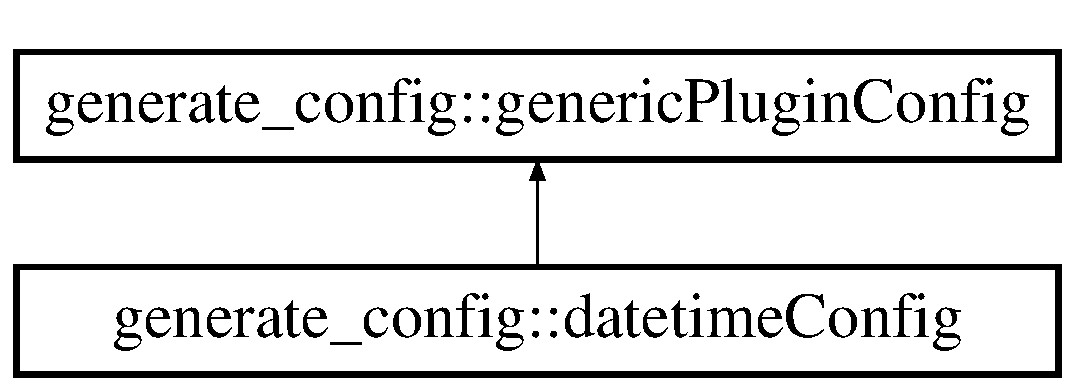
\includegraphics[height=2cm]{classgenerate__config_1_1datetimeConfig}
\end{center}
\end{figure}
\subsection*{Public Member Functions}
\begin{CompactItemize}
\item 
\hypertarget{classgenerate__config_1_1datetimeConfig_84bd0d1f10cb05b3513a3da208cab7bb}{
def \textbf{\_\-\_\-init\_\-\_\-}}
\label{classgenerate__config_1_1datetimeConfig_84bd0d1f10cb05b3513a3da208cab7bb}

\end{CompactItemize}


\subsection{Detailed Description}
Ask the user for specific config for the xPL datetime module. 

The documentation for this class was generated from the following file:\begin{CompactItemize}
\item 
config/generate\_\-config.py\end{CompactItemize}

\include{classdomogik_1_1doxypy_1_1FSM}
\hypertarget{classgenerate__config_1_1generalConfig}{
\section{generate\_\-config::generalConfig Class Reference}
\label{classgenerate__config_1_1generalConfig}\index{generate\_\-config::generalConfig@{generate\_\-config::generalConfig}}
}
Ask the user for general configuration and write results.  


\subsection*{Public Member Functions}
\begin{CompactItemize}
\item 
\hypertarget{classgenerate__config_1_1generalConfig_470de1124f102c64ad61af244dbac061}{
def \hyperlink{classgenerate__config_1_1generalConfig_470de1124f102c64ad61af244dbac061}{\_\-\_\-init\_\-\_\-}}
\label{classgenerate__config_1_1generalConfig_470de1124f102c64ad61af244dbac061}

\begin{CompactList}\small\item\em Ask user for general parameters of Domogik to create the main config file. \item\end{CompactList}\end{CompactItemize}


\subsection{Detailed Description}
Ask the user for general configuration and write results. 

The documentation for this class was generated from the following file:\begin{CompactItemize}
\item 
config/generate\_\-config.py\end{CompactItemize}

\hypertarget{classgenerate__config_1_1genericPluginConfig}{
\section{generate\_\-config::genericPluginConfig Class Reference}
\label{classgenerate__config_1_1genericPluginConfig}\index{generate\_\-config::genericPluginConfig@{generate\_\-config::genericPluginConfig}}
}
Inheritance diagram for generate\_\-config::genericPluginConfig::\begin{figure}[H]
\begin{center}
\leavevmode
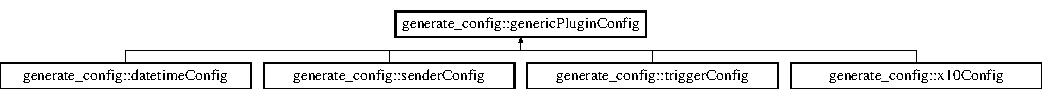
\includegraphics[height=1.20172cm]{classgenerate__config_1_1genericPluginConfig}
\end{center}
\end{figure}
\subsection*{Public Member Functions}
\begin{CompactItemize}
\item 
\hypertarget{classgenerate__config_1_1genericPluginConfig_6e5142c1890303123b37a9b1015601c8}{
def \textbf{\_\-\_\-init\_\-\_\-}}
\label{classgenerate__config_1_1genericPluginConfig_6e5142c1890303123b37a9b1015601c8}

\item 
\hypertarget{classgenerate__config_1_1genericPluginConfig_5e6843b1a07f91051930ac9ae93f4494}{
def \textbf{askandwrite}}
\label{classgenerate__config_1_1genericPluginConfig_5e6843b1a07f91051930ac9ae93f4494}

\end{CompactItemize}
\subsection*{Public Attributes}
\begin{CompactItemize}
\item 
\hypertarget{classgenerate__config_1_1genericPluginConfig_4d6143782994ef3d177b90f38f4512c4}{
\textbf{informations}}
\label{classgenerate__config_1_1genericPluginConfig_4d6143782994ef3d177b90f38f4512c4}

\end{CompactItemize}


\subsection{Detailed Description}


\footnotesize\begin{verbatim}
Generic list for plugins
\end{verbatim}
\normalsize
 

The documentation for this class was generated from the following file:\begin{CompactItemize}
\item 
config/generate\_\-config.py\end{CompactItemize}

\hypertarget{classxPLAPI_1_1Listener}{
\section{xPLAPI::Listener Class Reference}
\label{classxPLAPI_1_1Listener}\index{xPLAPI::Listener@{xPLAPI::Listener}}
}
\hyperlink{classxPLAPI_1_1Listener}{Listener} are objects which are able to check if a message match some filter and to call a function if they do.  




\subsection{Detailed Description}
\hyperlink{classxPLAPI_1_1Listener}{Listener} are objects which are able to check if a message match some filter and to call a function if they do. 

The documentation for this class was generated from the following file:\begin{CompactItemize}
\item 
xpl/xPLAPI.py\end{CompactItemize}

\include{classtrigger_1_1ListenerBuilder}
\hypertarget{classconfigloader_1_1Loader}{
\section{configloader::Loader Class Reference}
\label{classconfigloader_1_1Loader}\index{configloader::Loader@{configloader::Loader}}
}
Parse Domogik config files.  


\subsection*{Public Member Functions}
\begin{CompactItemize}
\item 
def \hyperlink{classconfigloader_1_1Loader_f16abb85a49b17461dcc647f4a2d5e00}{\_\-\_\-init\_\-\_\-}
\begin{CompactList}\small\item\em Load the configuration for a part of the Domogik system. \item\end{CompactList}\item 
def \hyperlink{classconfigloader_1_1Loader_52f1433b0ea290e45661b7473c3a68d4}{load}
\begin{CompactList}\small\item\em Parse the config. \item\end{CompactList}\end{CompactItemize}
\subsection*{Public Attributes}
\begin{CompactItemize}
\item 
\hypertarget{classconfigloader_1_1Loader_1a7a816df2d21c388cbb544c79caa065}{
\textbf{main\_\-conf\_\-name}}
\label{classconfigloader_1_1Loader_1a7a816df2d21c388cbb544c79caa065}

\item 
\hypertarget{classconfigloader_1_1Loader_44604dd7b77716499655a4f39453a13d}{
\textbf{module\_\-name}}
\label{classconfigloader_1_1Loader_44604dd7b77716499655a4f39453a13d}

\end{CompactItemize}


\subsection{Detailed Description}
Parse Domogik config files. 

\subsection{Member Function Documentation}
\hypertarget{classconfigloader_1_1Loader_f16abb85a49b17461dcc647f4a2d5e00}{
\index{configloader::Loader@{configloader::Loader}!\_\-\_\-init\_\-\_\-@{\_\-\_\-init\_\-\_\-}}
\index{\_\-\_\-init\_\-\_\-@{\_\-\_\-init\_\-\_\-}!configloader::Loader@{configloader::Loader}}
\subsubsection[\_\-\_\-init\_\-\_\-]{\setlength{\rightskip}{0pt plus 5cm}def configloader::Loader::\_\-\_\-init\_\-\_\- ( {\em self}, \/   {\em module\_\-name} = {\tt None})}}
\label{classconfigloader_1_1Loader_f16abb85a49b17461dcc647f4a2d5e00}


Load the configuration for a part of the Domogik system. 

\begin{Desc}
\item[Parameters:]
\begin{description}
\item[{\em module\_\-name}]name of the module to load config from \end{description}
\end{Desc}
\hypertarget{classconfigloader_1_1Loader_52f1433b0ea290e45661b7473c3a68d4}{
\index{configloader::Loader@{configloader::Loader}!load@{load}}
\index{load@{load}!configloader::Loader@{configloader::Loader}}
\subsubsection[load]{\setlength{\rightskip}{0pt plus 5cm}def configloader::Loader::load ( {\em self})}}
\label{classconfigloader_1_1Loader_52f1433b0ea290e45661b7473c3a68d4}


Parse the config. 

\begin{Desc}
\item[Returns:]pair (main\_\-config, plugin\_\-config) \end{Desc}


The documentation for this class was generated from the following file:\begin{CompactItemize}
\item 
xpl/configloader.py\end{CompactItemize}

\hypertarget{classxPLAPI_1_1Manager}{
\section{xPLAPI::Manager Class Reference}
\label{classxPLAPI_1_1Manager}\index{xPLAPI::Manager@{xPLAPI::Manager}}
}
\hyperlink{classxPLAPI_1_1Manager}{Manager} is the main component of the system You can run many managers on different port Each manager will send an heartbeat message on broadcast on port 3865 to announce itself to the xPL Hub.  




\subsection{Detailed Description}
\hyperlink{classxPLAPI_1_1Manager}{Manager} is the main component of the system You can run many managers on different port Each manager will send an heartbeat message on broadcast on port 3865 to announce itself to the xPL Hub. 

The documentation for this class was generated from the following file:\begin{CompactItemize}
\item 
xpl/xPLAPI.py\end{CompactItemize}

\hypertarget{classxPLAPI_1_1Message}{
\section{xPLAPI::Message Class Reference}
\label{classxPLAPI_1_1Message}\index{xPLAPI::Message@{xPLAPI::Message}}
}
\subsection*{Public Member Functions}
\begin{CompactItemize}
\item 
def \hyperlink{classxPLAPI_1_1Message_f1efb1186af373f1ce3d107be47e3f3f}{\_\-\_\-init\_\-\_\-}
\item 
def \hyperlink{classxPLAPI_1_1Message_a24b962cfffbd90f1cb79a2c20e581e6}{set\_\-type}
\item 
def \hyperlink{classxPLAPI_1_1Message_55aad8c9b685e349f7e3d3f58b6ff5aa}{get\_\-type}
\item 
def \hyperlink{classxPLAPI_1_1Message_560b2b7685ee99a34ea7d01e7135477c}{set\_\-schema}
\item 
def \hyperlink{classxPLAPI_1_1Message_58df48b064cb3d59780a51c67136e88a}{get\_\-schema}
\item 
def \hyperlink{classxPLAPI_1_1Message_014808e1035dcea973692d4d823427ce}{set\_\-conf\_\-key}
\item 
def \hyperlink{classxPLAPI_1_1Message_6bc039067bf79dd06b649e95870cfba9}{set\_\-data\_\-key}
\item 
def \hyperlink{classxPLAPI_1_1Message_254a763505a2ddb64ecd8d1b96f984d6}{set\_\-data\_\-order}
\item 
def \hyperlink{classxPLAPI_1_1Message_191e86e1dccd20aa0ea63158429e6d68}{set\_\-conf\_\-order}
\item 
def \hyperlink{classxPLAPI_1_1Message_e8bde03ac8436238c97cad324897c2ee}{has\_\-key}
\item 
def \hyperlink{classxPLAPI_1_1Message_8bc93e1bab48128e660be2d1e8ac7199}{has\_\-conf\_\-key}
\item 
def \hyperlink{classxPLAPI_1_1Message_80231e4e96a2247263ed3d2bb7f9cbf3}{get\_\-key\_\-value}
\item 
def \hyperlink{classxPLAPI_1_1Message_de17ca84597e627ae63f9b1cf5a4b284}{get\_\-conf\_\-key\_\-value}
\item 
\hypertarget{classxPLAPI_1_1Message_4d5b950513dedc31dfe0dcf51823c43d}{
def \textbf{\_\-\_\-str\_\-\_\-}}
\label{classxPLAPI_1_1Message_4d5b950513dedc31dfe0dcf51823c43d}

\end{CompactItemize}
\subsection*{Private Attributes}
\begin{CompactItemize}
\item 
\hypertarget{classxPLAPI_1_1Message_24328ca4d71be4d24f67d043d1c58f54}{
\textbf{\_\-conf}}
\label{classxPLAPI_1_1Message_24328ca4d71be4d24f67d043d1c58f54}

\item 
\hypertarget{classxPLAPI_1_1Message_29972dfac0cce8db6bd4a6a88adbe817}{
\textbf{\_\-data}}
\label{classxPLAPI_1_1Message_29972dfac0cce8db6bd4a6a88adbe817}

\item 
\hypertarget{classxPLAPI_1_1Message_88e4d23012224e9a9fa6ace6357016cb}{
\textbf{\_\-conf\_\-order}}
\label{classxPLAPI_1_1Message_88e4d23012224e9a9fa6ace6357016cb}

\item 
\hypertarget{classxPLAPI_1_1Message_9b6bd7b6c391434890d4ba996c3cda37}{
\textbf{\_\-data\_\-order}}
\label{classxPLAPI_1_1Message_9b6bd7b6c391434890d4ba996c3cda37}

\item 
\hypertarget{classxPLAPI_1_1Message_d4c56a71254ebbfc52582819bdc0c2d7}{
\textbf{\_\-type}}
\label{classxPLAPI_1_1Message_d4c56a71254ebbfc52582819bdc0c2d7}

\item 
\hypertarget{classxPLAPI_1_1Message_0f504647b076c8e1d4330941ee30f66f}{
\textbf{\_\-schema}}
\label{classxPLAPI_1_1Message_0f504647b076c8e1d4330941ee30f66f}

\end{CompactItemize}
\subsection*{Static Private Attributes}
\begin{CompactItemize}
\item 
\hypertarget{classxPLAPI_1_1Message_cd58199e9068e7351ac49b73675311f5}{
list \textbf{\_\-mess\_\-types} = \mbox{[}'xpl-stat','xpl-cmnd','xpl-trig'\mbox{]}}
\label{classxPLAPI_1_1Message_cd58199e9068e7351ac49b73675311f5}

\end{CompactItemize}


\subsection{Detailed Description}


\footnotesize\begin{verbatim}
Message is the object for all data received form the network.
The monitor create an instance of Message each time it receive smthg
\end{verbatim}
\normalsize
 

\subsection{Member Function Documentation}
\hypertarget{classxPLAPI_1_1Message_f1efb1186af373f1ce3d107be47e3f3f}{
\index{xPLAPI::Message@{xPLAPI::Message}!\_\-\_\-init\_\-\_\-@{\_\-\_\-init\_\-\_\-}}
\index{\_\-\_\-init\_\-\_\-@{\_\-\_\-init\_\-\_\-}!xPLAPI::Message@{xPLAPI::Message}}
\subsubsection[\_\-\_\-init\_\-\_\-]{\setlength{\rightskip}{0pt plus 5cm}def xPLAPI::Message::\_\-\_\-init\_\-\_\- ( {\em self}, \/   {\em mess} = {\tt None})}}
\label{classxPLAPI_1_1Message_f1efb1186af373f1ce3d107be47e3f3f}




\footnotesize\begin{verbatim}
Create Message instance from a message string and check if the structure 
is correct. Raise exception if it is not
The message can be None (to allow building a message)
@param mess : the message as a unique string, as it is send on the network
\end{verbatim}
\normalsize
 \hypertarget{classxPLAPI_1_1Message_a24b962cfffbd90f1cb79a2c20e581e6}{
\index{xPLAPI::Message@{xPLAPI::Message}!set\_\-type@{set\_\-type}}
\index{set\_\-type@{set\_\-type}!xPLAPI::Message@{xPLAPI::Message}}
\subsubsection[set\_\-type]{\setlength{\rightskip}{0pt plus 5cm}def xPLAPI::Message::set\_\-type ( {\em self}, \/   {\em type})}}
\label{classxPLAPI_1_1Message_a24b962cfffbd90f1cb79a2c20e581e6}




\footnotesize\begin{verbatim}
Define the message type (xpl-stat, xpl-trig or xpl-cmnd)
\end{verbatim}
\normalsize
 \hypertarget{classxPLAPI_1_1Message_55aad8c9b685e349f7e3d3f58b6ff5aa}{
\index{xPLAPI::Message@{xPLAPI::Message}!get\_\-type@{get\_\-type}}
\index{get\_\-type@{get\_\-type}!xPLAPI::Message@{xPLAPI::Message}}
\subsubsection[get\_\-type]{\setlength{\rightskip}{0pt plus 5cm}def xPLAPI::Message::get\_\-type ( {\em self})}}
\label{classxPLAPI_1_1Message_55aad8c9b685e349f7e3d3f58b6ff5aa}




\footnotesize\begin{verbatim}
Return the message type
\end{verbatim}
\normalsize
 \hypertarget{classxPLAPI_1_1Message_560b2b7685ee99a34ea7d01e7135477c}{
\index{xPLAPI::Message@{xPLAPI::Message}!set\_\-schema@{set\_\-schema}}
\index{set\_\-schema@{set\_\-schema}!xPLAPI::Message@{xPLAPI::Message}}
\subsubsection[set\_\-schema]{\setlength{\rightskip}{0pt plus 5cm}def xPLAPI::Message::set\_\-schema ( {\em self}, \/   {\em schema})}}
\label{classxPLAPI_1_1Message_560b2b7685ee99a34ea7d01e7135477c}




\footnotesize\begin{verbatim}
Define the message schema
\end{verbatim}
\normalsize
 \hypertarget{classxPLAPI_1_1Message_58df48b064cb3d59780a51c67136e88a}{
\index{xPLAPI::Message@{xPLAPI::Message}!get\_\-schema@{get\_\-schema}}
\index{get\_\-schema@{get\_\-schema}!xPLAPI::Message@{xPLAPI::Message}}
\subsubsection[get\_\-schema]{\setlength{\rightskip}{0pt plus 5cm}def xPLAPI::Message::get\_\-schema ( {\em self})}}
\label{classxPLAPI_1_1Message_58df48b064cb3d59780a51c67136e88a}




\footnotesize\begin{verbatim}
Return the message schema
\end{verbatim}
\normalsize
 \hypertarget{classxPLAPI_1_1Message_014808e1035dcea973692d4d823427ce}{
\index{xPLAPI::Message@{xPLAPI::Message}!set\_\-conf\_\-key@{set\_\-conf\_\-key}}
\index{set\_\-conf\_\-key@{set\_\-conf\_\-key}!xPLAPI::Message@{xPLAPI::Message}}
\subsubsection[set\_\-conf\_\-key]{\setlength{\rightskip}{0pt plus 5cm}def xPLAPI::Message::set\_\-conf\_\-key ( {\em self}, \/   {\em key}, \/   {\em value})}}
\label{classxPLAPI_1_1Message_014808e1035dcea973692d4d823427ce}




\footnotesize\begin{verbatim}
Define a configuration key (which appears between first {})
\end{verbatim}
\normalsize
 \hypertarget{classxPLAPI_1_1Message_6bc039067bf79dd06b649e95870cfba9}{
\index{xPLAPI::Message@{xPLAPI::Message}!set\_\-data\_\-key@{set\_\-data\_\-key}}
\index{set\_\-data\_\-key@{set\_\-data\_\-key}!xPLAPI::Message@{xPLAPI::Message}}
\subsubsection[set\_\-data\_\-key]{\setlength{\rightskip}{0pt plus 5cm}def xPLAPI::Message::set\_\-data\_\-key ( {\em self}, \/   {\em key}, \/   {\em value})}}
\label{classxPLAPI_1_1Message_6bc039067bf79dd06b649e95870cfba9}




\footnotesize\begin{verbatim}
Define a data key (which appears between second {})
\end{verbatim}
\normalsize
 \hypertarget{classxPLAPI_1_1Message_254a763505a2ddb64ecd8d1b96f984d6}{
\index{xPLAPI::Message@{xPLAPI::Message}!set\_\-data\_\-order@{set\_\-data\_\-order}}
\index{set\_\-data\_\-order@{set\_\-data\_\-order}!xPLAPI::Message@{xPLAPI::Message}}
\subsubsection[set\_\-data\_\-order]{\setlength{\rightskip}{0pt plus 5cm}def xPLAPI::Message::set\_\-data\_\-order ( {\em self}, \/   {\em order})}}
\label{classxPLAPI_1_1Message_254a763505a2ddb64ecd8d1b96f984d6}




\footnotesize\begin{verbatim}
As schema define parameter order, and since this class isn't specific enough to determine order,
you have to set the order to ensure a good message.
If you do not, the order of parameter in each part may not conform to schema
If you set order, be sure to list all the keys !
\end{verbatim}
\normalsize
 \hypertarget{classxPLAPI_1_1Message_191e86e1dccd20aa0ea63158429e6d68}{
\index{xPLAPI::Message@{xPLAPI::Message}!set\_\-conf\_\-order@{set\_\-conf\_\-order}}
\index{set\_\-conf\_\-order@{set\_\-conf\_\-order}!xPLAPI::Message@{xPLAPI::Message}}
\subsubsection[set\_\-conf\_\-order]{\setlength{\rightskip}{0pt plus 5cm}def xPLAPI::Message::set\_\-conf\_\-order ( {\em self}, \/   {\em order})}}
\label{classxPLAPI_1_1Message_191e86e1dccd20aa0ea63158429e6d68}




\footnotesize\begin{verbatim}
As schema define parameter order, and since this class isn't specific enough to determine order,
you have to set the order to ensure a good message.
If you do not, the order of parameter in each part may not conform to schema
If you set order, be sure to list all the keys !
\end{verbatim}
\normalsize
 \hypertarget{classxPLAPI_1_1Message_e8bde03ac8436238c97cad324897c2ee}{
\index{xPLAPI::Message@{xPLAPI::Message}!has\_\-key@{has\_\-key}}
\index{has\_\-key@{has\_\-key}!xPLAPI::Message@{xPLAPI::Message}}
\subsubsection[has\_\-key]{\setlength{\rightskip}{0pt plus 5cm}def xPLAPI::Message::has\_\-key ( {\em self}, \/   {\em key})}}
\label{classxPLAPI_1_1Message_e8bde03ac8436238c97cad324897c2ee}




\footnotesize\begin{verbatim}
Check if a key exists in data dictionnary
\end{verbatim}
\normalsize
 \hypertarget{classxPLAPI_1_1Message_8bc93e1bab48128e660be2d1e8ac7199}{
\index{xPLAPI::Message@{xPLAPI::Message}!has\_\-conf\_\-key@{has\_\-conf\_\-key}}
\index{has\_\-conf\_\-key@{has\_\-conf\_\-key}!xPLAPI::Message@{xPLAPI::Message}}
\subsubsection[has\_\-conf\_\-key]{\setlength{\rightskip}{0pt plus 5cm}def xPLAPI::Message::has\_\-conf\_\-key ( {\em self}, \/   {\em key})}}
\label{classxPLAPI_1_1Message_8bc93e1bab48128e660be2d1e8ac7199}




\footnotesize\begin{verbatim}
Check if a key exists in configuration dictionnary
\end{verbatim}
\normalsize
 \hypertarget{classxPLAPI_1_1Message_80231e4e96a2247263ed3d2bb7f9cbf3}{
\index{xPLAPI::Message@{xPLAPI::Message}!get\_\-key\_\-value@{get\_\-key\_\-value}}
\index{get\_\-key\_\-value@{get\_\-key\_\-value}!xPLAPI::Message@{xPLAPI::Message}}
\subsubsection[get\_\-key\_\-value]{\setlength{\rightskip}{0pt plus 5cm}def xPLAPI::Message::get\_\-key\_\-value ( {\em self}, \/   {\em key})}}
\label{classxPLAPI_1_1Message_80231e4e96a2247263ed3d2bb7f9cbf3}




\footnotesize\begin{verbatim}
get the value of a key from data
\end{verbatim}
\normalsize
 \hypertarget{classxPLAPI_1_1Message_de17ca84597e627ae63f9b1cf5a4b284}{
\index{xPLAPI::Message@{xPLAPI::Message}!get\_\-conf\_\-key\_\-value@{get\_\-conf\_\-key\_\-value}}
\index{get\_\-conf\_\-key\_\-value@{get\_\-conf\_\-key\_\-value}!xPLAPI::Message@{xPLAPI::Message}}
\subsubsection[get\_\-conf\_\-key\_\-value]{\setlength{\rightskip}{0pt plus 5cm}def xPLAPI::Message::get\_\-conf\_\-key\_\-value ( {\em self}, \/   {\em key})}}
\label{classxPLAPI_1_1Message_de17ca84597e627ae63f9b1cf5a4b284}




\footnotesize\begin{verbatim}
get the value of a key from configuration
\end{verbatim}
\normalsize
 

The documentation for this class was generated from the following file:\begin{CompactItemize}
\item 
xpl/xPLAPI.py\end{CompactItemize}

\include{classtrigger_1_1NOT}
\hypertarget{classonewire_1_1OneWire}{
\section{onewire::OneWire Class Reference}
\label{classonewire_1_1OneWire}\index{onewire::OneWire@{onewire::OneWire}}
}
Manage \hyperlink{classonewire_1_1OneWire}{OneWire}.  


\subsection*{Public Member Functions}
\begin{CompactItemize}
\item 
def \hyperlink{classonewire_1_1OneWire_effc317af881a97edf6d7dd77c63b88c}{\_\-\_\-init\_\-\_\-}
\begin{CompactList}\small\item\em Create \hyperlink{classonewire_1_1OneWire}{OneWire} instance, allowing to use \hyperlink{classonewire_1_1OneWire}{OneWire} Network. \item\end{CompactList}\item 
def \hyperlink{classonewire_1_1OneWire_41228b6b8c1562f02d0b40c8e40d96b4}{set\_\-cache\_\-use}
\begin{CompactList}\small\item\em Define use of cache. \item\end{CompactList}\item 
\hypertarget{classonewire_1_1OneWire_8c52e866328b82976eb9f799f891f487}{
def \hyperlink{classonewire_1_1OneWire_8c52e866328b82976eb9f799f891f487}{exec\_\-type}}
\label{classonewire_1_1OneWire_8c52e866328b82976eb9f799f891f487}

\begin{CompactList}\small\item\em Find all sensors matching a type. \item\end{CompactList}\item 
\hypertarget{classonewire_1_1OneWire_db399d215bf72b5084d5cbbefbdd62a9}{
def \hyperlink{classonewire_1_1OneWire_db399d215bf72b5084d5cbbefbdd62a9}{exec\_\-name}}
\label{classonewire_1_1OneWire_db399d215bf72b5084d5cbbefbdd62a9}

\begin{CompactList}\small\item\em Find all sensors matching a name. \item\end{CompactList}\item 
\hypertarget{classonewire_1_1OneWire_23324150ab22b72b6c32054003b400fd}{
def \hyperlink{classonewire_1_1OneWire_23324150ab22b72b6c32054003b400fd}{exec\_\-family}}
\label{classonewire_1_1OneWire_23324150ab22b72b6c32054003b400fd}

\begin{CompactList}\small\item\em Find all sensors matching a family. \item\end{CompactList}\item 
def \hyperlink{classonewire_1_1OneWire_ece120e9964b38335bf23a7028d45083}{get\_\-temperature}
\begin{CompactList}\small\item\em Return list of all temperature indicated by DS18B20 and DS18S20 sensors. \item\end{CompactList}\item 
\hypertarget{classonewire_1_1OneWire_a39fa5e62e0d65e62a915eb334d54fed}{
def \hyperlink{classonewire_1_1OneWire_a39fa5e62e0d65e62a915eb334d54fed}{is\_\-present}}
\label{classonewire_1_1OneWire_a39fa5e62e0d65e62a915eb334d54fed}

\begin{CompactList}\small\item\em Check if an item is on the network, and if it is, check if the present property is set to 1. \item\end{CompactList}\end{CompactItemize}
\subsection*{Private Attributes}
\begin{CompactItemize}
\item 
\hypertarget{classonewire_1_1OneWire_40f37588fd8a7fb0ac894db039ce1957}{
\textbf{\_\-root\_\-cached}}
\label{classonewire_1_1OneWire_40f37588fd8a7fb0ac894db039ce1957}

\item 
\hypertarget{classonewire_1_1OneWire_e2458b6e1c97fa036e57367bacdfe2d5}{
\textbf{\_\-root\_\-uncached}}
\label{classonewire_1_1OneWire_e2458b6e1c97fa036e57367bacdfe2d5}

\item 
\hypertarget{classonewire_1_1OneWire_f75836fcd181ffa0e98c7d3e5b9c25af}{
\textbf{\_\-cache}}
\label{classonewire_1_1OneWire_f75836fcd181ffa0e98c7d3e5b9c25af}

\item 
\hypertarget{classonewire_1_1OneWire_1165b31792f0a8955d26b55d524f58bf}{
\textbf{\_\-root}}
\label{classonewire_1_1OneWire_1165b31792f0a8955d26b55d524f58bf}

\end{CompactItemize}


\subsection{Detailed Description}
Manage \hyperlink{classonewire_1_1OneWire}{OneWire}. 

\subsection{Member Function Documentation}
\hypertarget{classonewire_1_1OneWire_effc317af881a97edf6d7dd77c63b88c}{
\index{onewire::OneWire@{onewire::OneWire}!\_\-\_\-init\_\-\_\-@{\_\-\_\-init\_\-\_\-}}
\index{\_\-\_\-init\_\-\_\-@{\_\-\_\-init\_\-\_\-}!onewire::OneWire@{onewire::OneWire}}
\subsubsection[\_\-\_\-init\_\-\_\-]{\setlength{\rightskip}{0pt plus 5cm}def onewire::OneWire::\_\-\_\-init\_\-\_\- ( {\em self}, \/   {\em dev} = {\tt 'u'})}}
\label{classonewire_1_1OneWire_effc317af881a97edf6d7dd77c63b88c}


Create \hyperlink{classonewire_1_1OneWire}{OneWire} instance, allowing to use \hyperlink{classonewire_1_1OneWire}{OneWire} Network. 

\begin{Desc}
\item[Parameters:]
\begin{description}
\item[{\em dev}]: device where the interface is connected to, default 'u' for USB \end{description}
\end{Desc}
\hypertarget{classonewire_1_1OneWire_41228b6b8c1562f02d0b40c8e40d96b4}{
\index{onewire::OneWire@{onewire::OneWire}!set\_\-cache\_\-use@{set\_\-cache\_\-use}}
\index{set\_\-cache\_\-use@{set\_\-cache\_\-use}!onewire::OneWire@{onewire::OneWire}}
\subsubsection[set\_\-cache\_\-use]{\setlength{\rightskip}{0pt plus 5cm}def onewire::OneWire::set\_\-cache\_\-use ( {\em self}, \/   {\em use})}}
\label{classonewire_1_1OneWire_41228b6b8c1562f02d0b40c8e40d96b4}


Define use of cache. 

If it's set to False, information will be reactualised each time a request is done If it's true, the OWFS cache will be used (from 15s to 2 minutes of cache) \hypertarget{classonewire_1_1OneWire_ece120e9964b38335bf23a7028d45083}{
\index{onewire::OneWire@{onewire::OneWire}!get\_\-temperature@{get\_\-temperature}}
\index{get\_\-temperature@{get\_\-temperature}!onewire::OneWire@{onewire::OneWire}}
\subsubsection[get\_\-temperature]{\setlength{\rightskip}{0pt plus 5cm}def onewire::OneWire::get\_\-temperature ( {\em self})}}
\label{classonewire_1_1OneWire_ece120e9964b38335bf23a7028d45083}


Return list of all temperature indicated by DS18B20 and DS18S20 sensors. 

\begin{Desc}
\item[Returns:]list of (id, temperature) \end{Desc}


The documentation for this class was generated from the following file:\begin{CompactItemize}
\item 
xpl/onewire.py\end{CompactItemize}

\hypertarget{classonewire_1_1OneWireException}{
\section{onewire::OneWireException Class Reference}
\label{classonewire_1_1OneWireException}\index{onewire::OneWireException@{onewire::OneWireException}}
}
\hyperlink{classonewire_1_1OneWire}{OneWire} exception.  


\subsection*{Public Member Functions}
\begin{CompactItemize}
\item 
\hypertarget{classonewire_1_1OneWireException_e19dc9d7c1ad8e838679a1670ec20802}{
def \textbf{\_\-\_\-init\_\-\_\-}}
\label{classonewire_1_1OneWireException_e19dc9d7c1ad8e838679a1670ec20802}

\item 
\hypertarget{classonewire_1_1OneWireException_b97f5138487e792bca2b75f392cdd70d}{
def \textbf{\_\-\_\-str\_\-\_\-}}
\label{classonewire_1_1OneWireException_b97f5138487e792bca2b75f392cdd70d}

\end{CompactItemize}
\subsection*{Public Attributes}
\begin{CompactItemize}
\item 
\hypertarget{classonewire_1_1OneWireException_4e217e555112a6ddf7b601637a835571}{
\textbf{value}}
\label{classonewire_1_1OneWireException_4e217e555112a6ddf7b601637a835571}

\end{CompactItemize}


\subsection{Detailed Description}
\hyperlink{classonewire_1_1OneWire}{OneWire} exception. 

The documentation for this class was generated from the following file:\begin{CompactItemize}
\item 
xpl/onewire.py\end{CompactItemize}

\include{classtrigger_1_1OR}
\hypertarget{classdomogik_1_1control_1_1SampleDataHelper_1_1SampleDataHelper}{
\section{domogik::control::SampleDataHelper::SampleDataHelper Class Reference}
\label{classdomogik_1_1control_1_1SampleDataHelper_1_1SampleDataHelper}\index{domogik::control::SampleDataHelper::SampleDataHelper@{domogik::control::SampleDataHelper::SampleDataHelper}}
}
\subsection*{Public Member Functions}
\begin{CompactItemize}
\item 
\hypertarget{classdomogik_1_1control_1_1SampleDataHelper_1_1SampleDataHelper_8289ab362d8b5048a413e6c5b3d3f4de}{
def \textbf{remove}}
\label{classdomogik_1_1control_1_1SampleDataHelper_1_1SampleDataHelper_8289ab362d8b5048a413e6c5b3d3f4de}

\item 
\hypertarget{classdomogik_1_1control_1_1SampleDataHelper_1_1SampleDataHelper_72168a6303032d0742cc905fa2bb3a65}{
def \textbf{create}}
\label{classdomogik_1_1control_1_1SampleDataHelper_1_1SampleDataHelper_72168a6303032d0742cc905fa2bb3a65}

\end{CompactItemize}


\subsection{Detailed Description}


\footnotesize\begin{verbatim}
Class to load / clear sample data
\end{verbatim}
\normalsize
 

The documentation for this class was generated from the following file:\begin{CompactItemize}
\item 
control/SampleDataHelper.py\end{CompactItemize}

\hypertarget{classgenerate__config_1_1senderConfig}{
\section{generate\_\-config::senderConfig Class Reference}
\label{classgenerate__config_1_1senderConfig}\index{generate\_\-config::senderConfig@{generate\_\-config::senderConfig}}
}
Inheritance diagram for generate\_\-config::senderConfig::\begin{figure}[H]
\begin{center}
\leavevmode
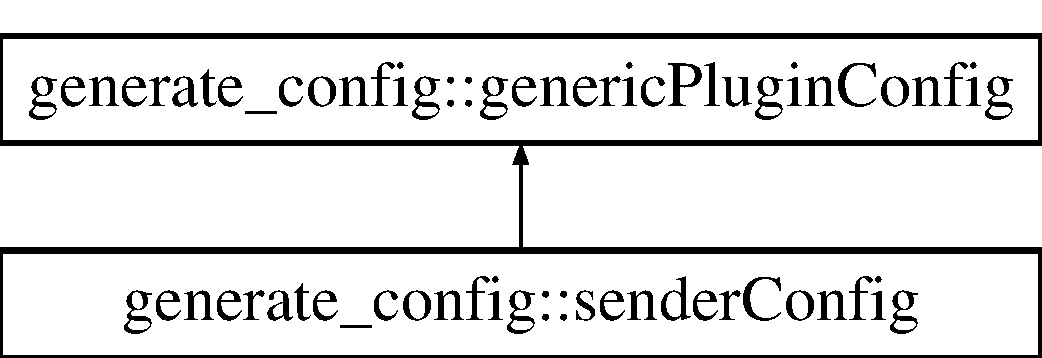
\includegraphics[height=2cm]{classgenerate__config_1_1senderConfig}
\end{center}
\end{figure}
\subsection*{Public Member Functions}
\begin{CompactItemize}
\item 
\hypertarget{classgenerate__config_1_1senderConfig_0eaa1e44dfc6199842d784e2211a6f67}{
def \textbf{\_\-\_\-init\_\-\_\-}}
\label{classgenerate__config_1_1senderConfig_0eaa1e44dfc6199842d784e2211a6f67}

\end{CompactItemize}


\subsection{Detailed Description}


\footnotesize\begin{verbatim}
Ask the user for specific config for the xPL sender
\end{verbatim}
\normalsize
 

The documentation for this class was generated from the following file:\begin{CompactItemize}
\item 
config/generate\_\-config.py\end{CompactItemize}

\include{classtrigger_1_1stateCond}
\include{classtrigger_1_1timeCond}
\hypertarget{classgenerate__config_1_1triggerConfig}{
\section{generate\_\-config::triggerConfig Class Reference}
\label{classgenerate__config_1_1triggerConfig}\index{generate\_\-config::triggerConfig@{generate\_\-config::triggerConfig}}
}
Ask the user for specific config for the xPL sender.  


Inheritance diagram for generate\_\-config::triggerConfig::\begin{figure}[H]
\begin{center}
\leavevmode
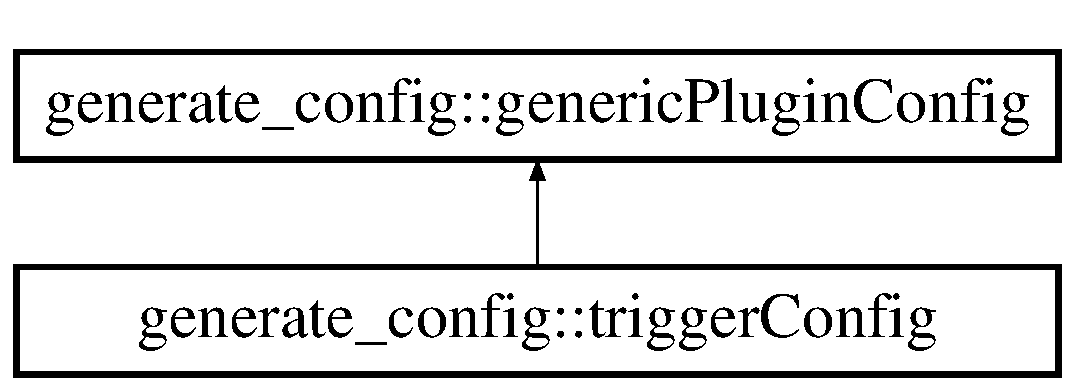
\includegraphics[height=2cm]{classgenerate__config_1_1triggerConfig}
\end{center}
\end{figure}
\subsection*{Public Member Functions}
\begin{CompactItemize}
\item 
\hypertarget{classgenerate__config_1_1triggerConfig_40e2f872feeb29963472a73ca7937dfd}{
def \textbf{\_\-\_\-init\_\-\_\-}}
\label{classgenerate__config_1_1triggerConfig_40e2f872feeb29963472a73ca7937dfd}

\end{CompactItemize}


\subsection{Detailed Description}
Ask the user for specific config for the xPL sender. 

The documentation for this class was generated from the following file:\begin{CompactItemize}
\item 
config/generate\_\-config.py\end{CompactItemize}

\hypertarget{classx10API_1_1X10API}{
\section{x10API::X10API Class Reference}
\label{classx10API_1_1X10API}\index{x10API::X10API@{x10API::X10API}}
}
\subsection*{Public Member Functions}
\begin{CompactItemize}
\item 
\hypertarget{classx10API_1_1X10API_df1708474fd2eda336c665c64067a648}{
def \textbf{\_\-\_\-init\_\-\_\-}}
\label{classx10API_1_1X10API_df1708474fd2eda336c665c64067a648}

\item 
def \hyperlink{classx10API_1_1X10API_b23095bb54aa45e75857beaa59a7deed}{on}
\item 
def \hyperlink{classx10API_1_1X10API_37be53c20aaa39f5770a5085b80984bc}{off}
\item 
def \hyperlink{classx10API_1_1X10API_d1e63a9dd573eb16a7d1009c72fac15e}{house\_\-on}
\item 
def \hyperlink{classx10API_1_1X10API_b04c7647aa5d80c462f0df36afaff4ec}{house\_\-off}
\end{CompactItemize}
\subsection*{Private Member Functions}
\begin{CompactItemize}
\item 
def \hyperlink{classx10API_1_1X10API_398d98e0674a6cefaef1154eafe94a15}{\_\-valid\_\-item}
\item 
def \hyperlink{classx10API_1_1X10API_e9639dcec52e0f507fcc224a6c377c7d}{\_\-valid\_\-house}
\item 
def \hyperlink{classx10API_1_1X10API_268f590bc14835490b1ea823c86e4dcb}{\_\-send}
\end{CompactItemize}
\subsection*{Private Attributes}
\begin{CompactItemize}
\item 
\hypertarget{classx10API_1_1X10API_e2bc653247758e1a67d8b8ac5b0d3611}{
\textbf{\_\-housecodes}}
\label{classx10API_1_1X10API_e2bc653247758e1a67d8b8ac5b0d3611}

\item 
\hypertarget{classx10API_1_1X10API_d2d5e02d43d6d4d1b0eba44248d29bb5}{
\textbf{\_\-unitcodes}}
\label{classx10API_1_1X10API_d2d5e02d43d6d4d1b0eba44248d29bb5}

\item 
\hypertarget{classx10API_1_1X10API_e11abda6663c0ad8d5e63d6abd52d562}{
\textbf{\_\-heyuconf}}
\label{classx10API_1_1X10API_e11abda6663c0ad8d5e63d6abd52d562}

\end{CompactItemize}


\subsection{Detailed Description}


\footnotesize\begin{verbatim}
This class define some facilities to use X10.
It's based on heyu software, you need to have it installed
and heyu binaries must be in your PATH
\end{verbatim}
\normalsize
 

\subsection{Member Function Documentation}
\hypertarget{classx10API_1_1X10API_398d98e0674a6cefaef1154eafe94a15}{
\index{x10API::X10API@{x10API::X10API}!\_\-valid\_\-item@{\_\-valid\_\-item}}
\index{\_\-valid\_\-item@{\_\-valid\_\-item}!x10API::X10API@{x10API::X10API}}
\subsubsection[\_\-valid\_\-item]{\setlength{\rightskip}{0pt plus 5cm}def x10API::X10API::\_\-valid\_\-item ( {\em self}, \/   {\em item})\hspace{0.3cm}{\tt  \mbox{[}private\mbox{]}}}}
\label{classx10API_1_1X10API_398d98e0674a6cefaef1154eafe94a15}




\footnotesize\begin{verbatim}
Check an item to have good 'HU' syntax
Raise exception if it is not
\end{verbatim}
\normalsize
 \hypertarget{classx10API_1_1X10API_e9639dcec52e0f507fcc224a6c377c7d}{
\index{x10API::X10API@{x10API::X10API}!\_\-valid\_\-house@{\_\-valid\_\-house}}
\index{\_\-valid\_\-house@{\_\-valid\_\-house}!x10API::X10API@{x10API::X10API}}
\subsubsection[\_\-valid\_\-house]{\setlength{\rightskip}{0pt plus 5cm}def x10API::X10API::\_\-valid\_\-house ( {\em self}, \/   {\em house})\hspace{0.3cm}{\tt  \mbox{[}private\mbox{]}}}}
\label{classx10API_1_1X10API_e9639dcec52e0f507fcc224a6c377c7d}




\footnotesize\begin{verbatim}
Check an house to have good 'H' syntax
Raise exception if it is not
\end{verbatim}
\normalsize
 \hypertarget{classx10API_1_1X10API_268f590bc14835490b1ea823c86e4dcb}{
\index{x10API::X10API@{x10API::X10API}!\_\-send@{\_\-send}}
\index{\_\-send@{\_\-send}!x10API::X10API@{x10API::X10API}}
\subsubsection[\_\-send]{\setlength{\rightskip}{0pt plus 5cm}def x10API::X10API::\_\-send ( {\em self}, \/   {\em cmd}, \/   {\em item})\hspace{0.3cm}{\tt  \mbox{[}private\mbox{]}}}}
\label{classx10API_1_1X10API_268f590bc14835490b1ea823c86e4dcb}




\footnotesize\begin{verbatim}
Send a command trought heyu
@param cmd : Command to send ('ON','OFF', etc)
@param item : Item to send order to (Can be HU or H form)
\end{verbatim}
\normalsize
 \hypertarget{classx10API_1_1X10API_b23095bb54aa45e75857beaa59a7deed}{
\index{x10API::X10API@{x10API::X10API}!on@{on}}
\index{on@{on}!x10API::X10API@{x10API::X10API}}
\subsubsection[on]{\setlength{\rightskip}{0pt plus 5cm}def x10API::X10API::on ( {\em self}, \/   {\em item})}}
\label{classx10API_1_1X10API_b23095bb54aa45e75857beaa59a7deed}




\footnotesize\begin{verbatim}
Send an ON order to the item element
@param item : the item to send the ON order to
@Return True if order was sent, False in case of errors
\end{verbatim}
\normalsize
 \hypertarget{classx10API_1_1X10API_37be53c20aaa39f5770a5085b80984bc}{
\index{x10API::X10API@{x10API::X10API}!off@{off}}
\index{off@{off}!x10API::X10API@{x10API::X10API}}
\subsubsection[off]{\setlength{\rightskip}{0pt plus 5cm}def x10API::X10API::off ( {\em self}, \/   {\em item})}}
\label{classx10API_1_1X10API_37be53c20aaa39f5770a5085b80984bc}




\footnotesize\begin{verbatim}
Send an OFF order to the item element
@param item : the item to send the OFF order to
@Return True if order was sent, False in case of errors
\end{verbatim}
\normalsize
 \hypertarget{classx10API_1_1X10API_d1e63a9dd573eb16a7d1009c72fac15e}{
\index{x10API::X10API@{x10API::X10API}!house\_\-on@{house\_\-on}}
\index{house\_\-on@{house\_\-on}!x10API::X10API@{x10API::X10API}}
\subsubsection[house\_\-on]{\setlength{\rightskip}{0pt plus 5cm}def x10API::X10API::house\_\-on ( {\em self}, \/   {\em house})}}
\label{classx10API_1_1X10API_d1e63a9dd573eb16a7d1009c72fac15e}




\footnotesize\begin{verbatim}
Send an ALLON order to the item element
@param item : the item to send the ALLON order to
@Return True if order was sent, False in case of errors
\end{verbatim}
\normalsize
 \hypertarget{classx10API_1_1X10API_b04c7647aa5d80c462f0df36afaff4ec}{
\index{x10API::X10API@{x10API::X10API}!house\_\-off@{house\_\-off}}
\index{house\_\-off@{house\_\-off}!x10API::X10API@{x10API::X10API}}
\subsubsection[house\_\-off]{\setlength{\rightskip}{0pt plus 5cm}def x10API::X10API::house\_\-off ( {\em self}, \/   {\em house})}}
\label{classx10API_1_1X10API_b04c7647aa5d80c462f0df36afaff4ec}




\footnotesize\begin{verbatim}
Send an ALLOFF order to the item element
@param item : the item to send the ALLOFF order to
@Return True if order was sent, False in case of errors
\end{verbatim}
\normalsize
 

The documentation for this class was generated from the following file:\begin{CompactItemize}
\item 
xpl/x10API.py\end{CompactItemize}

\hypertarget{classgenerate__config_1_1x10Config}{
\section{generate\_\-config::x10Config Class Reference}
\label{classgenerate__config_1_1x10Config}\index{generate\_\-config::x10Config@{generate\_\-config::x10Config}}
}
Ask the user for specific config for X10 xPL module.  


Inheritance diagram for generate\_\-config::x10Config::\begin{figure}[H]
\begin{center}
\leavevmode
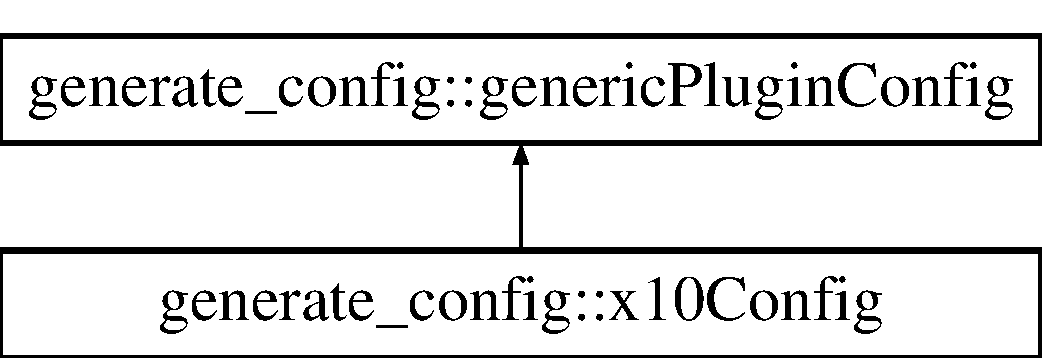
\includegraphics[height=2cm]{classgenerate__config_1_1x10Config}
\end{center}
\end{figure}
\subsection*{Public Member Functions}
\begin{CompactItemize}
\item 
\hypertarget{classgenerate__config_1_1x10Config_ebb61db62b6f7df09e9061255514bb70}{
def \textbf{\_\-\_\-init\_\-\_\-}}
\label{classgenerate__config_1_1x10Config_ebb61db62b6f7df09e9061255514bb70}

\end{CompactItemize}


\subsection{Detailed Description}
Ask the user for specific config for X10 xPL module. 

The documentation for this class was generated from the following file:\begin{CompactItemize}
\item 
config/generate\_\-config.py\end{CompactItemize}

\hypertarget{classx10API_1_1X10Exception}{
\section{x10API::X10Exception Class Reference}
\label{classx10API_1_1X10Exception}\index{x10API::X10Exception@{x10API::X10Exception}}
}
X10 exception.  


\subsection*{Public Member Functions}
\begin{CompactItemize}
\item 
\hypertarget{classx10API_1_1X10Exception_033a895f90bdb03c500be02471701831}{
def \textbf{\_\-\_\-init\_\-\_\-}}
\label{classx10API_1_1X10Exception_033a895f90bdb03c500be02471701831}

\item 
\hypertarget{classx10API_1_1X10Exception_a9a0adf2ba11276fecd3d7d0f759a8c9}{
def \textbf{\_\-\_\-str\_\-\_\-}}
\label{classx10API_1_1X10Exception_a9a0adf2ba11276fecd3d7d0f759a8c9}

\end{CompactItemize}
\subsection*{Public Attributes}
\begin{CompactItemize}
\item 
\hypertarget{classx10API_1_1X10Exception_ea0d93a4bd33db7e6f416fe28d739c84}{
\textbf{value}}
\label{classx10API_1_1X10Exception_ea0d93a4bd33db7e6f416fe28d739c84}

\end{CompactItemize}


\subsection{Detailed Description}
X10 exception. 

The documentation for this class was generated from the following file:\begin{CompactItemize}
\item 
xpl/x10API.py\end{CompactItemize}

\hypertarget{classdatetime_1_1xPLDateTime}{
\section{datetime::xPLDateTime Class Reference}
\label{classdatetime_1_1xPLDateTime}\index{datetime::xPLDateTime@{datetime::xPLDateTime}}
}
\subsection*{Public Member Functions}
\begin{CompactItemize}
\item 
\hypertarget{classdatetime_1_1xPLDateTime_b39a3cb860ddd3595e348bc7f910f1e4}{
def \textbf{\_\-\_\-init\_\-\_\-}}
\label{classdatetime_1_1xPLDateTime_b39a3cb860ddd3595e348bc7f910f1e4}

\end{CompactItemize}
\subsection*{Private Member Functions}
\begin{CompactItemize}
\item 
def \hyperlink{classdatetime_1_1xPLDateTime_56f581af02f2f66b6b8d21fe910b9b5d}{\_\-f}
\item 
def \hyperlink{classdatetime_1_1xPLDateTime_8705cd0ed46a76dda2d82c1a87fc1b3e}{\_\-send\_\-datetime}
\end{CompactItemize}
\subsection*{Private Attributes}
\begin{CompactItemize}
\item 
\hypertarget{classdatetime_1_1xPLDateTime_1b15c71df12789d777f44dc8d39e48f9}{
\textbf{\_\-\_\-myxpl}}
\label{classdatetime_1_1xPLDateTime_1b15c71df12789d777f44dc8d39e48f9}

\item 
\hypertarget{classdatetime_1_1xPLDateTime_7d66e43fe5cd70d3e9c8a90ae406dcc7}{
\textbf{\_\-timer}}
\label{classdatetime_1_1xPLDateTime_7d66e43fe5cd70d3e9c8a90ae406dcc7}

\end{CompactItemize}


\subsection{Detailed Description}


\footnotesize\begin{verbatim}
Send date and time on the xPL network every minute
\end{verbatim}
\normalsize
 

\subsection{Member Function Documentation}
\hypertarget{classdatetime_1_1xPLDateTime_56f581af02f2f66b6b8d21fe910b9b5d}{
\index{datetime::xPLDateTime@{datetime::xPLDateTime}!\_\-f@{\_\-f}}
\index{\_\-f@{\_\-f}!datetime::xPLDateTime@{datetime::xPLDateTime}}
\subsubsection[\_\-f]{\setlength{\rightskip}{0pt plus 5cm}def datetime::xPLDateTime::\_\-f ( {\em self}, \/   {\em nb})\hspace{0.3cm}{\tt  \mbox{[}private\mbox{]}}}}
\label{classdatetime_1_1xPLDateTime_56f581af02f2f66b6b8d21fe910b9b5d}




\footnotesize\begin{verbatim}
Format the number
\end{verbatim}
\normalsize
 \hypertarget{classdatetime_1_1xPLDateTime_8705cd0ed46a76dda2d82c1a87fc1b3e}{
\index{datetime::xPLDateTime@{datetime::xPLDateTime}!\_\-send\_\-datetime@{\_\-send\_\-datetime}}
\index{\_\-send\_\-datetime@{\_\-send\_\-datetime}!datetime::xPLDateTime@{datetime::xPLDateTime}}
\subsubsection[\_\-send\_\-datetime]{\setlength{\rightskip}{0pt plus 5cm}def datetime::xPLDateTime::\_\-send\_\-datetime ( {\em self})\hspace{0.3cm}{\tt  \mbox{[}private\mbox{]}}}}
\label{classdatetime_1_1xPLDateTime_8705cd0ed46a76dda2d82c1a87fc1b3e}




\footnotesize\begin{verbatim}
Send date and time on xPL network
\end{verbatim}
\normalsize
 

The documentation for this class was generated from the following file:\begin{CompactItemize}
\item 
xpl/datetime.py\end{CompactItemize}

\hypertarget{classxPLAPI_1_1XPLException}{
\section{xPLAPI::XPLException Class Reference}
\label{classxPLAPI_1_1XPLException}\index{xPLAPI::XPLException@{xPLAPI::XPLException}}
}
xPL exception  


\subsection*{Public Member Functions}
\begin{CompactItemize}
\item 
\hypertarget{classxPLAPI_1_1XPLException_fa97cb40136ea6f52c5b9ce792435e75}{
def \textbf{\_\-\_\-init\_\-\_\-}}
\label{classxPLAPI_1_1XPLException_fa97cb40136ea6f52c5b9ce792435e75}

\item 
\hypertarget{classxPLAPI_1_1XPLException_2713888a5319bbbeb96a991547dd127b}{
def \textbf{\_\-\_\-str\_\-\_\-}}
\label{classxPLAPI_1_1XPLException_2713888a5319bbbeb96a991547dd127b}

\end{CompactItemize}
\subsection*{Public Attributes}
\begin{CompactItemize}
\item 
\hypertarget{classxPLAPI_1_1XPLException_a426e1d994b5f51ef4249260b8357de7}{
\textbf{value}}
\label{classxPLAPI_1_1XPLException_a426e1d994b5f51ef4249260b8357de7}

\end{CompactItemize}


\subsection{Detailed Description}
xPL exception 

The documentation for this class was generated from the following file:\begin{CompactItemize}
\item 
xpl/xPLAPI.py\end{CompactItemize}

\hypertarget{classxPLAPI_1_1xPLTimer}{
\section{xPLAPI::xPLTimer Class Reference}
\label{classxPLAPI_1_1xPLTimer}\index{xPLAPI::xPLTimer@{xPLAPI::xPLTimer}}
}
\subsection*{Public Member Functions}
\begin{CompactItemize}
\item 
def \hyperlink{classxPLAPI_1_1xPLTimer_e651d6889d77aabd9227e622d5821d14}{\_\-\_\-init\_\-\_\-}
\item 
def \hyperlink{classxPLAPI_1_1xPLTimer_f9e579ecf5a8e2b2ed86ce78c5029a0e}{start}
\item 
def \hyperlink{classxPLAPI_1_1xPLTimer_2a04504c8d29908bc6601879fe63aa23}{stop}
\end{CompactItemize}
\subsection*{Private Member Functions}
\begin{CompactItemize}
\item 
def \hyperlink{classxPLAPI_1_1xPLTimer_59ac53c691fadf44bf28fb74a226251f}{\_\-run}
\end{CompactItemize}
\subsection*{Private Attributes}
\begin{CompactItemize}
\item 
\hypertarget{classxPLAPI_1_1xPLTimer_cf45a98a98a98ce25ae50665771d1e92}{
\textbf{\_\-callback}}
\label{classxPLAPI_1_1xPLTimer_cf45a98a98a98ce25ae50665771d1e92}

\item 
\hypertarget{classxPLAPI_1_1xPLTimer_a5189f41b3d558ccef9411af7c563796}{
\textbf{\_\-time}}
\label{classxPLAPI_1_1xPLTimer_a5189f41b3d558ccef9411af7c563796}

\item 
\hypertarget{classxPLAPI_1_1xPLTimer_f2a85e94f12015c68fb34b4461476cc3}{
\textbf{\_\-timer}}
\label{classxPLAPI_1_1xPLTimer_f2a85e94f12015c68fb34b4461476cc3}

\end{CompactItemize}


\subsection{Detailed Description}


\footnotesize\begin{verbatim}
xPLTimer will call a callback function each n seconds
\end{verbatim}
\normalsize
 

\subsection{Member Function Documentation}
\hypertarget{classxPLAPI_1_1xPLTimer_e651d6889d77aabd9227e622d5821d14}{
\index{xPLAPI::xPLTimer@{xPLAPI::xPLTimer}!\_\-\_\-init\_\-\_\-@{\_\-\_\-init\_\-\_\-}}
\index{\_\-\_\-init\_\-\_\-@{\_\-\_\-init\_\-\_\-}!xPLAPI::xPLTimer@{xPLAPI::xPLTimer}}
\subsubsection[\_\-\_\-init\_\-\_\-]{\setlength{\rightskip}{0pt plus 5cm}def xPLAPI::xPLTimer::\_\-\_\-init\_\-\_\- ( {\em self}, \/   {\em time}, \/   {\em cb})}}
\label{classxPLAPI_1_1xPLTimer_e651d6889d77aabd9227e622d5821d14}




\footnotesize\begin{verbatim}
Constructor : create the internal timer
@param time : time of loop in second
@param cb : callback function which will be call eact 'time' seconds
\end{verbatim}
\normalsize
 \hypertarget{classxPLAPI_1_1xPLTimer_59ac53c691fadf44bf28fb74a226251f}{
\index{xPLAPI::xPLTimer@{xPLAPI::xPLTimer}!\_\-run@{\_\-run}}
\index{\_\-run@{\_\-run}!xPLAPI::xPLTimer@{xPLAPI::xPLTimer}}
\subsubsection[\_\-run]{\setlength{\rightskip}{0pt plus 5cm}def xPLAPI::xPLTimer::\_\-run ( {\em self})\hspace{0.3cm}{\tt  \mbox{[}private\mbox{]}}}}
\label{classxPLAPI_1_1xPLTimer_59ac53c691fadf44bf28fb74a226251f}




\footnotesize\begin{verbatim}
internal timer loopback function
\end{verbatim}
\normalsize
 \hypertarget{classxPLAPI_1_1xPLTimer_f9e579ecf5a8e2b2ed86ce78c5029a0e}{
\index{xPLAPI::xPLTimer@{xPLAPI::xPLTimer}!start@{start}}
\index{start@{start}!xPLAPI::xPLTimer@{xPLAPI::xPLTimer}}
\subsubsection[start]{\setlength{\rightskip}{0pt plus 5cm}def xPLAPI::xPLTimer::start ( {\em self})}}
\label{classxPLAPI_1_1xPLTimer_f9e579ecf5a8e2b2ed86ce78c5029a0e}




\footnotesize\begin{verbatim}
Start the timer
\end{verbatim}
\normalsize
 \hypertarget{classxPLAPI_1_1xPLTimer_2a04504c8d29908bc6601879fe63aa23}{
\index{xPLAPI::xPLTimer@{xPLAPI::xPLTimer}!stop@{stop}}
\index{stop@{stop}!xPLAPI::xPLTimer@{xPLAPI::xPLTimer}}
\subsubsection[stop]{\setlength{\rightskip}{0pt plus 5cm}def xPLAPI::xPLTimer::stop ( {\em self})}}
\label{classxPLAPI_1_1xPLTimer_2a04504c8d29908bc6601879fe63aa23}




\footnotesize\begin{verbatim}
Stop the timer
\end{verbatim}
\normalsize
 

The documentation for this class was generated from the following file:\begin{CompactItemize}
\item 
xpl/xPLAPI.py\end{CompactItemize}

\printindex
\end{document}
